%Simon Krenger: Diskrete Mathematik
\documentclass{report}
\usepackage{amsmath}
\usepackage{amsthm}
\usepackage{amssymb}
\usepackage[utf8]{inputenc} 
\usepackage{graphicx}

\newtheorem{mydef}{Definition}
\newtheorem{myexample}{Beispiel}
\newtheorem{myproof}{Beweis}
\newtheorem{axiom}{Axiom}

\title{Diskrete Mathematik}
\author{Simon Krenger, Christian Meyer}

\begin{document}
\maketitle
\chapter{Logik (Boolesche Algebra)}
Nach George Bool, 1815 bis 1864, Cork (Irland)
\section{Aussagen}
Wir betrachten Aussagen (Sätze), die entweder wahr (1) oder falsch (0) sind.

\begin{quote}Heute ist Freitag \(\to\) wahr\end{quote}
\begin{quote}Morgen schneit es in Bern \(\to\) falsch\end{quote}
\begin{quote}Schauen Sie einmal! \(\to\) keine Aussage\end{quote}
Aussagen bezeichnen wir mit a, b, c, d, …
\begin{mydef}
Ist a eine Aussage, somit heisst  \(\lnot\)a die \underline{Negation} von a
\end{mydef}
\begin{myexample}a: Xaver isst gerne Kuchen
\(\lnot\)a: Xaver isst nicht gerne Kuchen\end{myexample}

\section{Konjunktion}
Wir verbinden zwei Aussagen a, b mit Hilfe von “und” zu einer einzigen Aussage
\begin{equation}a \land b\end{equation}
\begin{myexample}Morgen ist Sonntag \underline{und} ich werde ausschlafen\end{myexample}

Die Wahrheitstabelle von a \(\land\) b sind abhängig von denjenigen von a als auch von b. Dies stellen wir in einer \underline{Wahrheitswerttabelle} dar. Wir finden sofort die Regeln
\begin{equation}a \land \lnot a = falsch\end{equation}


\begin{mydef}Eine Aussage, die immer falsch ist, heisst \underline{Kontradiktion}.\end{mydef}

\begin{equation}a \land 1 = a\end{equation}
\begin{equation}a \land 0 = 0\end{equation}
Weiter finden wir Gesetze
\begin{quote}Kommutativgesetz (Vertauschungsgesetz)\end{quote}
\begin{equation}a \land b = b \land a\end{equation}
\begin{myproof}Wir beweisen mit einer Wahrheitswerttabelle
\begin{center}\begin{tabular}{c c | c c}
a & b & a \(\land\) b & b \(\land\) a\\
\hline
0 & 0 & 0 & 0  \\
0 & 1 & 0 & 0  \\
1 & 0 & 0 & 0 \\
1 & 1 & 1 & 1 \\
\end{tabular}\end{center}\end{myproof}
\begin{quote}Assoziativgesetz (Verbindungsgesetz)\end{quote}
\begin{equation}a \land (b \land c) = (a \land b) \land c\end{equation}
\begin{myproof}Wir beweisen mit einer Wahrheitswerttabelle
\begin{center}\begin{tabular}{c c c | c c}
a & b & c & a \(\land\) (b \(\land\) c) & (a \(\land\) b) \(\land\) c\\
\hline
0 & 0 & 0 & 0 & 0  \\
0 & 0 & 1 & 0 & 0  \\
0 & 1 & 0 & 0 & 0 \\
0 & 1 & 1 & 0 & 0 \\
1 & 0 & 0 & 0 & 0 \\
1 & 0 & 1 & 0 & 0 \\
1 & 1 & 0 & 0 & 0 \\
1 & 1 & 1 & 1 & 1 \\
\end{tabular}\end{center}\end{myproof}
\begin{quote}Idempotenzgesetz\end{quote}
\begin{equation}a \land a = a\end{equation}
\section{Disjunktion}
Zwei Aussagen a, b werden mit der Disjunktion "oder" zu einer neuen Aussage verbunden. Dafür schreiben wir:\begin{equation}a \lor b\end{equation}
und definieren
\begin{center}\begin{tabular}{c c | c}
a & b & a \(\lor\) b\\
\hline
0 & 0 & 0  \\
0 & 1 & 1  \\
1 & 0 & 1 \\
1 & 1 & 1 \\
\end{tabular}\end{center}
Nicht verwechseln mit "entweder oder" (XOR)! Wir finden die Regeln
\begin{equation}a \lor 1 = 1\end{equation}
\begin{equation}a \lor 0 = a\end{equation}
\begin{equation}a \lor \lnot a = 1\end{equation}
\begin{mydef}Eine Aussage, die stets wahr ist, heisst \underline{Tautologie}.\end{mydef}
Es gelten die Gesetze
\begin{quote}Kommutativgesetz\end{quote}
\begin{equation}a \lor b = b \lor a\end{equation}
\begin{quote}Assoziativgesetz\end{quote}
\begin{equation}a \lor (b \lor c) = (a \lor b) \lor c\end{equation}
\begin{quote}Idempotenzgesetz\end{quote}
\begin{equation}a \lor a = a\end{equation}
In der Algebra in \(\mathbb{R}\) gilt
\begin{equation}a(b+c) = ab+ac\end{equation}
was in der Logik zu
\begin{equation} \label{eq:distributivgesetz}a \land (b \lor c) = (a \land b) \lor (a \land c)\end{equation}
\begin{equation}a \lor (b \land c) = (a \lor b) \land (a \lor c)\end{equation}
dem \underline{Distributivgesetz} (Verteilungsgesetz) führt. Der folgende Beweis zeigt, dass die Gleichung \ref{eq:distributivgesetz} gilt.
\begin{myproof}Wir beweisen mit einer Wahrheitswerttabelle
\begin{center}\begin{tabular}{c c c | c c c c c}
a & b & c & b \(\lor\) c & a \(\land\) (b \(\lor\) c) & a \(\land\) b & a \(\land\) c & (a \(\land\) b) \(\lor\) (a \(\land\) c)  \\
\hline
0 & 0 & 0 & 0 & 0 & 0 & 0 & 0  \\
0 & 0 & 1 & 1 & 0 & 0 & 0 & 0  \\
0 & 1 & 0 & 1 & 0 & 0 & 0 & 0 \\
0 & 1 & 1 & 1 & 0 & 0 & 0 & 0 \\
1 & 0 & 0 & 0 & 0 & 0 & 0 & 0 \\
1 & 0 & 1 & 1 & 1 & 0 & 1 & 1 \\
1 & 1 & 0 & 1 & 1 & 1 & 0 & 1 \\
1 & 1 & 1 & 1 & 1 & 1 & 1 & 1 \\
\end{tabular}\end{center}
Das zweite Distributivgesetz kann analog dazu bewiesen werden.\end{myproof}
In der Logik gibt es zu jedem Gesetz ein \underline{duales Gesetz}. Dies entsteht durch wechseln von \(\lor\) zu \(\land\) und umgekehrt. Weiter finden wir
\begin{quote}Absorbtionsgesetz\end{quote}
\begin{equation}a \land (a \lor b) = a\end{equation}
\begin{equation}a \lor (a \land b) = a\end{equation}
\begin{myproof}Wir beweisen mit einer Wahrheitswerttabelle
\begin{center}\begin{tabular}{c c | c c}
a & b & a \(\lor\) b & a \(\land\) (a \(\lor\) b) \\
\hline
0 & 0 & 0 & 0  \\
0 & 1 & 1 & 0  \\
1 & 0 & 1 & 1  \\
1 & 1 & 1 & 1 \\
\end{tabular}\end{center}\end{myproof}
\begin{quote}Gesetz von de Morgan\end{quote}
\begin{equation}\lnot (a \land b) = \lnot a \lor \lnot b\end{equation}
\begin{equation}\lnot (a \lor b) = \lnot a \land \lnot b\end{equation}
Wir verwenden die Gesetze, um die Aussagen zu vereinfachen.
\begin{myexample}Folgende Beispiele zeigen, wie sich Aussagen mittels den oben genannten Gesetzen vereinfachen lassen.
\begin{enumerate}
\item $[a \land (b \lor a)] \lor \lnot a$\\
$= a \lor \lnot a$\\
$= 1$
\item $[\lnot (a \land b) \lor \lnot b] \land a$\\
$= (\lnot a \lor \lnot b \lor \lnot b) \land a$\\
$= (\lnot a \lor \lnot b) \land a$\\
$= (\lnot a \land a) \lor (\lnot b \land a)$\\
$= 0 \lor (\lnot b \land a)$\\
$= \lnot b \land a$
\item $(a \land b) \lor \lnot b$\\
$= (a \lor \lnot b) \land (b \lor \lnot b)$\\
$= (a \lor \lnot b) \land 1$\\
$= (a \lor \lnot b)$
\item $b \land [(a \land b) \lor ( \lnot a \land b)]$\\
$= b \land [b \land (a \lor \lnot a)]$\\
$= b \land (b \land 1)$\\
$= b \land b = b$
\end{enumerate}
\end{myexample}
\section{Implikation}
Mathematische Lehrsätze haben die Form "Wenn ein Dreieck rechtwinklig ist mit Hypothenuse $c$ und Katheten $a$, $b$, dann ist $c^2=a^2+b^2$"\\
Sie bestehen also aus Voraussetzung(en):
\begin{quote}Das Dreieck ist rechtwinklig\end{quote}
und Behauptung
\begin{quote}Es ist $a^2+b^2=c^2$\end{quote}
und einem Beweis
\begin{quote}\begin{proof}[Beweis] Gemäss "Indischer Beweis":
\begin{eqnarray}c^2&=&4\frac{ab}{2}+(a-b)^2 \nonumber \\
c^2&=&2ab+a^2-2ab+b^2\nonumber \\
c^2&=&a^2+b^2\end{eqnarray}\end{proof}\end{quote}
Im obrigen Beispiel haben wir einen direkten Beweis geführt. Von der Voraussetzung durch Rechnung zur Behauptung.\\
Wenn wir zwei Aussagen a, b mit "wenn a, dann b" oder "wenn a so b" oder "aus a folgt b (a impliziert b)" verknüpfen, so schreiben wir dafür
\begin{equation}a \to b\end{equation}
und definieren
\begin{center}\begin{tabular}{c c | c}
a & b & a \(\to\) b\\
\hline
0 & 0 & 1  \\
0 & 1 & 1  \\
1 & 0 & 0 \\
1 & 1 & 1 \\
\end{tabular}\end{center}
Wir finden sofort, das "aus a folgt b"
\begin{equation}a \to b = \lnot a \lor b\end{equation}
\begin{myexample}Vereinfache
\begin{enumerate}
\item $(a \to b) \to b$\\
$= (\lnot a \lor b) \to b = \lnot(\lnot a \lor b) \lor b$\\
$= (a \land \lnot b) \lor b = (a \lor b) \land (\lnot b \lor b)$\\
$= (a \lor b) \land 1 = (a \lor b)$
\item $b \to (a \to b)$\\
$= b \to (\lnot a \lor b) = \lnot b \lor (\lnot a \lor b)$\\
$= \lnot b \lor b \lor \lnot a = 1 \lor \lnot a = 1$
\item $[(a \lor c) \land (c \to a)] \lor (a \land \lnot b) \lor (a \land c) \lor [\lnot a \land (b \to c)]$\\
$=[(a \lor c) \land (\lnot c \lor a)] \lor (a \land \lnot b) \lor (a \land c) \lor [\lnot a \land (\lnot b \lor c)]$\\
$=[(a \lor c) \land (\lnot c \lor a)] \lor [a \land (\lnot v \lor c)] \lor [\lnot a \land (\lnot b \lor c)]$\\
$=[a \lor (c \land \lnot c)] \lor [(\lnot b \lor c) \land (a \lor \lnot a)]$\\
$=[a \lor 0] \lor [(\lnot b \lor c) \land 1]$\\
$=a \lor (\lnot v \lor c) = a \lor \lnot b \lor c$\\
$(=a \lor (b \to c))$
\end{enumerate}
\end{myexample}
Ein mathematischer Satz besteht aus Voraussetzung $a$, Behauptung $b$ und Beweis. Der Satz wird als $a \to b$ formuliert.\\
Der direkte Beweis ist eine Folge von Implikationen
\begin{equation}a \to x_1 \to x_2 \to x_3 \to ... \to b\end{equation}
\begin{myexample}Vereinfache
\begin{enumerate}
\item Voraussetzung: Ein Dreieck ABC mit Innenwinkel $\alpha$, $\beta$, $\gamma$\\
Behauptung: Die Innenwinkelsumme ist $180^{\circ}$, d.h. 
\begin{equation}\alpha+\beta+\gamma=180^{\circ}\end{equation}
\begin{proof}[Beweis]Wir beweisen mit einer Zeichnung:\begin{center}
\includegraphics[scale=0.5]{img/innenwinkel.png}
\end{center}
Wähle $p \parallel c$ durch C. Dann ist $\epsilon+\delta+\gamma=180^{\circ}$. Es ist $\alpha_1$= $\alpha_2$: Stufenwinkel an Parallelen und $\alpha_1$= $\alpha_3$: Wechselwinkel an Parallelen, eine weitere Voraussetzung.\\
Also ist $\alpha = \epsilon$ und $\beta = \delta$
und somit
\begin{equation}\alpha+\beta+\gamma=180^{\circ}\end{equation}
\end{proof}
\item Voraussetzung: Es ist mit $n \in \mathbb{N}, a \in \mathbb{R}$
\begin{center}$a^n := a \cdot a \cdot ... \cdot a$ (n Faktoren)\end{center}
die Potenz definiert.
Behauptung: \begin{equation}a^m \cdot a^n = a^{m+n}\end{equation}
\begin{proof}[Beweis]Wir zeigen auf, dass $m$ Faktoren mit $n$ Faktoren multipliziert werden. Durch die grundlegenden Rechengesetze können wir die Klammern wegfallen lassen
\begin{center}$a^m \cdot a^n$\\
$= (a \cdot a \cdot a \cdot ... \cdot a)(a \cdot a \cdot ... \cdot a)$\\
$= a \cdot a \cdot a \cdot a \cdot ... \cdot a$ (m+n Faktoren)\end{center}
\begin{equation}= a^{m+n} = a^m \cdot a^n\end{equation}
\end{proof}
\item \label{item:gegenbeispiel} Voraussetzung: $x, y \in \mathbb{R}$\\
Behauptung: \begin{equation} x^y = y^x \to x = y\end{equation} 
Die Behauptung ist falsch. Wollen wir zeigen, dass ein Satz falsch ist, so genügt ein einziges Beispiel, dass wir \underline{Gegenbeispiel} nennen, um die Behauptung zu widerlegen.\\
Gegenbeispiel: Für \ref{item:gegenbeispiel} ist das Gegenbeispiel $x=2, y=4$, denn $2^4 = 4^2 = 16$, aber $x \neq y$.
\end{enumerate}
\end{myexample}

\subsection{Umkehrung, Kontraposition}
\begin{mydef}Hat eine Aussage die Form
\begin{equation}a \to b\end{equation}
so heisst
\begin{equation}b \to a\end{equation}
die \underline{Umkehrung}.
\end{mydef}
Ist eine Aussage, ein Satz wahr, so muss die Umkehrung nicht wahr sein, wie zum Beispiel:
\begin{quote}"Wenn ich Geburtstag habe, so esse ich einen Kuchen"\end{quote}
\begin{quote}"Wenn ein Mensch glücklich ist, so trinkt er Sinalco"\end{quote}
Wir finden aber, dass
\begin{eqnarray}\lnot b \to \lnot a = \lnot(\lnot b) \lor \lnot a \nonumber\\
= b \lor \lnot a = \lnot a \lor b = a \to b\end{eqnarray}
\begin{mydef}Wir nennen
\begin{equation}\lnot b \to \lnot a\end{equation}
die \underline{Kontraposition} von
\begin{equation}a \to b\end{equation}
\end{mydef}
Wir haben gezeigt, dass $\lnot b \to \lnot a = a \to b$ ist, was bedeutet, dass bei einem wahren Satz auch dessen Kontraposition wahr ist.
\begin{quote}{Satz}: "Wenn es heute Freitag ist, so gehe ich ein Bier trinken."\end{quote}
\begin{quote}{Kontraposition}: "Wenn ich nicht ein Bier trinken gehe, so ist heute Freitag"\end{quote}
Manchmal ist der direkte Beweis eines Satzes zu schwierig oder nicht möglich, dann beweisen wir die Kontraposition.
\begin{quote}{Satz}: Ist $n \in \mathbb{N}$ und $n^2$ eine gerade Zahl, so ist $n$ auch eine gerade Zahl.\end{quote}
\begin{myproof}Der direkte Beweis
\begin{eqnarray}n^2 &=& 2p \land p \in \mathbb{N} \nonumber \\
\to n &=& \sqrt{2} \cdot \sqrt{p}\end{eqnarray}
gelingt nicht. Grund dafür ist, dass eine irrationale Zahl ($\sqrt{2}$) per Definition ein nichtperiodischer, nichtendlicher Dezimalbruch ist.\end{myproof}
Also beweisen wir die Kontraposition:
\begin{quote}{Kontraposition}: "Ist $n \in \mathbb{N}$ und $n$ ungerade, so ist auch $n^2$ ungerade"\end{quote}
\begin{myproof}\begin{eqnarray} 
n &=& 2p + 1 \quad \land p \in \mathbb{N}_0 \nonumber \\
\to n^2 &=& (2p + 1)^2 \nonumber \\
n^2 &=& 4p^2 + 4p + 1 \nonumber \\
n^2 &=& 2 (2p^2 + 2p) + 1\label{eq:nungerade} \end{eqnarray}
Also ist $n^2$ eine ungerade Zahl.\qed\end{myproof}

\section{Aequivalenz}
Wenn zwei Aussagen gleichwertig (aequivalent) sind, wenn also
\begin{equation}(a \to b) \land (b \to a)\end{equation}
so schreiben wir dafür
\begin{equation}a \iff b\end{equation}
und finden die Wahrheitswerte
\begin{center}\begin{tabular}{c c | c}
a & b & a \(\iff\) b\\
\hline
0 & 0 & 1 \\
0 & 1 & 0 \\
1 & 0 & 0 \\
1 & 1 & 1 \\
\end{tabular}\end{center}
Wir finden die Umformung
\begin{eqnarray}
a \iff b &=& (a \to b) \land (b \to a)\nonumber \\
&=& (\lnot a \lor b) \land (\lnot b \lor a)\nonumber \\
&=& (\lnot a \land b) \lor (\lnot a \land a) \lor (b \land \lnot b) \lor (a \land b) \nonumber \\
&=& (a \land b) \lor (\lnot a \land \lnot b)
\end{eqnarray}
Ausserdem ist 
\begin{equation}a \iff b = \lnot (a \veebar b)\end{equation}
also
\begin{eqnarray}a \veebar b &=& [(a \land b) \lor (\lnot a \land \lnot b)] \nonumber \\
&=&\lnot(a \land b) \land \lnot (\lnot a \land \lnot b) \nonumber \\
&=&(\lnot a \lor \lnot b) \land (a \lor b)\end{eqnarray}
\begin{myexample}Vereinfache
\begin{enumerate}
\item $(\lnot a \lor \lnot b) \land (a \lor b)$\\
$=a \veebar b$ nach obriger Herleitung
\item $(a \land \lnot b \land \lnot c) \lor (a \land b \land c)$\\
$= a \land [(\lnot b \land \lnot c) \lor (b \land c)]$\\
$= a \land (b \iff c)$
\end{enumerate}
\end{myexample}
Wenn wir in der Mathematik einen Satz finden, dessen Umkehrung auch wahr ist, so wählen wir die Formulierung mit
\begin{quote}"dann und nur dann" oder "genau dann"\end{quote}
im Englischen
\begin{quote}"if and only if" oder "iff"\end{quote}
\begin{myexample}Folgende Beispiele zeigen solche Sätze
\begin{enumerate}
\item Zwei Dreiecke $ABC$ und $A_1B_1C_1$ sind \underline{genau dann} ähnlich, \underline{wenn} zwei Winkel gleich sind.
%TODO: IMAGE
\item Sind $a$, $b$ reelle Zahlen, so ist das Produkt \underline{dann und nur dann} 0, \underline{wenn} $a$ oder $b$ Null ist.
\begin{quote}{Voraussetzung}: $a, b \in \mathbb{R}$\end{quote}
\begin{quote}{Satz}: $(a \cdot b = 0) \iff (a = 0 \lor b = 0)$\end{quote}
\begin{quote}{Anwendung}:\begin{eqnarray}a^2 - 7x + 12 &=& 0\quad(x \in \mathbb{R}) \nonumber \\
(x-3)(x-4)&=&0 \nonumber \\
\to x-3=0 \quad &\lor& \quad x-4=0 \nonumber \\
x_1 = 3 &\quad& x_2 = 4\end{eqnarray}\end{quote}
\end{enumerate}
\end{myexample}
Wie zeigen wir, dass zwei Terme gleich sind?
\begin{quote}{Behauptung}: \begin{equation}\sin{2\alpha} = 2\sin{\alpha}\cos{\alpha}\end{equation} \end{quote}
Wir wählen die linke Seite und formen diese so lange um, bis die rechte Seite entsteht (oder umgekehrt).\\Es ist \underline{falsch}
\begin{equation}\sin{2\alpha} = 2\sin{\alpha}\cos{\alpha}\end{equation}
so lange umzuformen, bis eine Identität wie z.B. $1 = 1$ entsteht!

\begin{myexample}Richtig ist
\begin{eqnarray}\sin{2\alpha} &=& \sin{\alpha + \alpha} \nonumber \\
\mbox{denn}\quad \sin{\alpha + \beta} &=& \sin{\alpha}\cos{\beta}+\sin{\beta}\cos{\alpha}\nonumber \\
\sin{\alpha + \alpha} &=& \sin{\alpha}\cos{\alpha}+\sin{\alpha}\cos{\alpha} \nonumber \\
&=& 2\sin{\alpha}\cos{\alpha}\end{eqnarray} \qed\end{myexample}
Manchmal gelingt es nicht, die linke Seite in die rechte Seite umzuformen. Dann verwenden wir die Eigenschaft
\begin{quote}"Wenn $l=x$ und $r=x$, so ist $l=r$\end{quote}
Wir formen also die linke Seite zuerst einmal um und dann \underline{unabhängig davon} die rechte Seite und hoffen, dass wir beide Male das gleiche Resultat ($x$) erhalten.
\begin{myexample}Wir versuchen, dieses Konzept anzuwenden:\\\\
Voraussetzung: \begin{equation}\tan{\delta} = \frac{\sin{\delta}}{\cos{\delta}} \quad\mbox{und}\quad\cot{\delta} = \frac{1}{\tan{\delta}}\end{equation}
Behauptung: \begin{equation}\tan{\delta} + \cot{\delta} = \frac{2}{\sin{2\delta}}\end{equation}
Beweis: \begin{enumerate}
\item \begin{eqnarray}& &\tan{\delta} + \frac{1}{\tan{\delta}}
=\frac{\sin{\delta}}{\cos{\delta}} + \frac{\cos{\delta}}{\sin{\delta}} \nonumber \\
&=&\frac{\sin^2{\delta} + \cos^2{\delta}}{\sin{\delta} \cdot \cos{\delta}} 
=\frac{1}{\sin{\delta} \cdot \cos{\delta}}\end{eqnarray}
\item \begin{eqnarray}& &\frac{2}{\sin{2\delta}} = \frac{2}{2\sin{\delta} \cdot \cos{\delta}}
=\frac{1}{\sin{\delta} \cdot \cos{\delta}}\end{eqnarray}\qed
\end{enumerate}\end{myexample}
Genau gleich behandeln wir Behauptungen der Logik wenn es um die Aequivalenz zweier Aussagen geht.
\begin{myexample}\begin{enumerate}
\item Behauptung: \begin{equation}[\lnot(a \lor b) \land a] \iff [\lnot (a \lor b) \land b]\end{equation}
Beweis:\begin{enumerate}
\item \begin{eqnarray}\lnot (a \lor b) \land a &=& \lnot a \land \lnot b \land a \nonumber \\
= \lnot a \land a \land \lnot b &=& 0 \land \lnot b = 0\end{eqnarray}
\item \begin{eqnarray}\lnot (a \lor b) \land b &=& \lnot a \land \lnot b \land b \nonumber \\
= \lnot a \land b \land \lnot b &=& \lnot a \land b = 0\end{eqnarray}\end{enumerate}Beide Terme sind aequivalent\qed
\item Behauptung: \begin{equation}a \to (b \land c) = (a \to b) \land (a \to c)\end{equation}
Beweis: \begin{eqnarray}\lnot a \lor (b \land c) &=& (\lnot a \lor b) \land (\lnot a \lor c) \nonumber \\
&=& (a \to b) \land (a \to c)\end{eqnarray}\end{enumerate}\end{myexample}

\section{Logische Schlüsse}
Wir gehen aus von verschiedenen \underline{Prämissen} wie
\begin{eqnarray}\mbox{Prämisse 1} & & p_1 = a \land b \nonumber \\
\mbox{Prämisse 2}& & p_2 = \lnot a \nonumber \\
\mbox{Prämisse 3}& & p_3 = a \land \lnot b\end{eqnarray}
und ziehen daraus eine \underline{Konklusion} $k : a \lor b$. Nun fragen wir uns, ob die Konklusion bei diesen Prämissen richtig ist. Ist dies der Fall, so sprechen wir von einem logischen Schluss (wenn also das die richtige Konklusion ist).
\\\\Es muss also
\begin{equation}(p_1 \land p_2 \land ... \land p_n) \to k = 1\end{equation}
eine Tautologie sein. Im Beispiel ist also
\begin{equation}[(a \land b) \land \lnot a \land (a \land \lnot b)] \to (a \lor b)\end{equation}
so lange umgeformt werden, bis erkenntlich ist, ob eine Tautologie vorliegt oder nicht.
\begin{eqnarray}& &[(a \land b) \land \lnot a \land (a \land \lnot b)] \to (a \lor b) \nonumber \\
&=&(a \land b \land \lnot a \land a \land \lnot b) \to (a \lor b) \nonumber \\
&=&0 \to (a \lor b) \nonumber \\
&=&\lnot 0 \lor (a \lor b) = 1 \lor (a \lor b) = 1\end{eqnarray}
und damit liegt ein logischer Schluss vor.\\\\
In der Logik schreiben wir Prämissen und Konklusion untereinander wie zum Beispiel
\begin{equation}\frac{a \to b \quad\quad a \land b \to c \quad\quad c}{a}\end{equation}
\begin{myexample}Handelt es sich hierbei um einen logischen Schluss?\begin{eqnarray}& &[(a \to b) \land \{(a \land b) \to c\} \land c] \to a \nonumber \\
&=&[(\lnot a \lor b) \land \{\lnot (a \land b) \lor c\} \land c] \to a \nonumber \\
&=&\lnot [(\lnot a \lor b) \land (\lnot a \lor \lnot b \lor c) \land c] \lor a \nonumber \\
&=&\lnot [(\lnot a \lor b) \land c] \lor a \nonumber \\
&=&\lnot [(\lnot a \land c) \lor (b \land c)] \lor a\nonumber \\
&=&[\lnot (\lnot a \land c) \land \lnot (b \land c)] \lor a \nonumber \\
&=&[(a \lor \lnot c) \land (\lnot b \lor \lnot c)] \lor a \nonumber \\
&=&(a \lor \lnot c \lor a) \land (a \lor \lnot b \lor \lnot c) \nonumber \\
&=&(\lnot c \lor a) \land (\lnot b \lor \lnot c \lor a) \nonumber \\
&=&(\lnot c \lor a) \land \lnot b\end{eqnarray}
Also kein logischer Schluss \qed\end{myexample}
Verschiedene bekannte logische Schlüsse besitzen einen Namen, wie zum Beispiel die Folgdenden:
\begin{enumerate}
\item \underline{modus ponens} (Abtrennungsregel)
\begin{equation}\frac{a \to b \quad\quad a}{b}\end{equation}
ist ein logischer Schluss, denn
\begin{eqnarray}& &[(a \to b) \land a] \to b \nonumber \\
&=&[(\lnot a \lor b) \land a] \to b \nonumber \\
&=&(a \land b) \to b \nonumber \\
&=&\lnot (a \land b) \lor b \nonumber \\
&=&\lnot a \lor \lnot b \lor b = \lnot a \lor 1 = 1\end{eqnarray}
Es ist die Art und Weise, wie wir einen mathematischen Satz $a \to b$ anwenden.
\begin{myexample}Beispielsweise Kosinussatz:\\
$a \to b$: In einem Dreieck $ABC$ gilt $c^2 = a^2 + b^2 - 2ab \cdot \cos{\gamma}$ \\
$a$: $a=10, b=7, \gamma = 70$\\
dann tritt $b$ ein, d.h. c kann nun berechnet werden.\end{myexample}
\item \underline{modus tollens} (Aufhebende Schlussweise)
\begin{equation}\frac{a \to b \quad\quad \lnot b}{\lnot a}\end{equation}
ist ein logischer Schluss, denn
\begin{eqnarray}& &[(a \to b) \land \lnot b] \to \lnot a \nonumber \\
&=&[(\lnot a \lor b) \land \lnot b] \to \lnot a \nonumber \\
&=&[(b \land \lnot b) \lor (\lnot a \land \lnot b)] \to \lnot a \nonumber \\
&=&(\lnot a \land \lnot b) \to \lnot a \nonumber \\
&=&\lnot (\lnot a \land \lnot b) \lor \lnot a \nonumber \\
&=&a \lor b \lor \lnot a = 1 \lor b = 1\end{eqnarray}
\item \underline{reductio ad absurdum} (zurückführen auf einen Widerspruch)
\begin{equation} \frac{a \to (b \land \lnot b)}{\lnot a}\end{equation}
ist ein logischer Schluss, denn
\begin{eqnarray}& &[a \to (b \land \lnot b)] \to \lnot a \nonumber \\
&=&[a \to 0] \to \lnot a \nonumber \\
&=&[\lnot a \lor 0] \to \lnot a \nonumber \\
&=&\lnot a \to \lnot a = a \lor \lnot a = 1\end{eqnarray}
Dieser logische Schluss führt uns zum \underline{Beweis mit Gegenannahme}.\\\\
Wollen wir beweisen, dass ein Satz $s$ wahr ist und gelingt uns dies nicht mit einem direkten Beweis oder mit einem Beweis mit Kontraposition, so wählen wir die Gegenannahme:
\begin{quote}$\lnot s$ ist wahr\end{quote}
und zeigen, dass dies zu einem Widerspruch führt wie $\lnot b \land b$ oder $1 = 2$ oder ähnlich.\\\\
Dann sagt uns die "reductio ad absurdum", dass meine Gegenannahme falsch ist und damit die Aussage $s$ wahr ist.\end{enumerate}
\begin{myexample}\begin{enumerate}
\item Satz: "Es gibt unendlich viele Primzahlen"\\
Beweis mit Gegenannahme (Euklid, ca. 300 v.Chr., Alexandria):
\begin{quote}"Es gibt nur endlich viele Primzahlen"\end{quote}
\begin{equation}p_1 < p_2 < p_3 < ... < p_{n-1} < p_n\end{equation}
wobei $p_n$ die Grösste sei.\\
Nun bilden wir eine neue Zahl
\begin{equation}z = p_1 \cdot p_2 \cdot p_3 \cdot ... \cdot p_n + 1\end{equation}
die sicher keine der Zahlen $p_1, p_2, p_3, ..., p_n$ als Primfaktoren besitzt.\\
Nun ist $z$ entweder
\begin{enumerate}\item eine Primzahl, dann ist dies ein Widerspruch
\item keine Primzahl und damit in Primfaktoren zerlegbar. Es muss also neben $p_1, p_2, ..., p_n$ einen weiteren Primfaktor geben, dies ist ein Widerspruch\end{enumerate}
zur Gegenannahme.\\
Also ist die Gegenannahme falsch und damit die ursprüngliche Behauptung wahr. \qed

\item Behauptung: $\sqrt{2}$ ist irrational\\
Beweis mit Gegenannahme:
\begin{quote}$\sqrt{2}$ ist rational\end{quote}
also ist $\sqrt{2} = \frac{p}{q} \land p, q \in \mathbb{N}$ und vollständig gekürzt. Somit
\begin{eqnarray}2&=&\frac{p^2}{q^2} \nonumber \\
p^2&=&2q^2 \label{eq:sqrtirrational} \end{eqnarray}
Also ist $p^2$ eine gerade Zahl und damit auch $p$ (Beweis siehe \ref{eq:nungerade}). Somit ist $p = 2x \land p \in \mathbb{N}$, was eingesetzt in \ref{eq:sqrtirrational} zu
\begin{equation}(2x)^2 = 2q^2\end{equation}
führt. Weiter ist
\begin{eqnarray}4x^2&=&2q^2 \nonumber \\
2x^2&=&q^2\end{eqnarray}
Also ist $q^2$ gerade und damit auch q. Somit ist
\begin{equation}q = 2y \land y \in \mathbb{N}\end{equation}
WIr haben also gefunden
\begin{equation}\sqrt{2} = \frac{p}{q} = \frac{2x}{2y}\end{equation}
und damit erhalten wir einen Widerspruch zu "vollständig gekürzt". Somit ist die Gegenannahme falsch und damit die Behauptung richtig.
\end{enumerate}\end{myexample}
Einen Beweis mit Gegenannahme nennen wir auch einen \underline{indirekten Beweis}. Dieses Beweisverfahren können wir auch für logische Schlüsse anwenden.\\\\
Ist
\begin{equation}\frac{a \land \lnot b \quad a \to b}{a \lor b}\end{equation}
ein logischer Schluss?
\begin{quote}Gegenannahme: Es ist liegt kein logischer Schluss vor und damit ist
\begin{equation}[(a \land \lnot b) \land (a \to b)] \to (a \lor b) = 0\end{equation}\end{quote}
Nun zeigen wir, dass die Gegenannahme zu einem Widerspruch führt. Wir haben die Aussage
\begin{equation}x \to y = 0 \nonumber\end{equation}
Also muss $x=1$ und $y=0$ sein.\\\\
Es ist $x = p_1 \land p_2 \land ... \land p_n$ (Alle Prämissen und damit muss auch
\begin{equation}p_1 = p_2 = ... = p_n = 1 \nonumber \end{equation}
sein. Um den Widerspruch zu sehen, machen wir eine Tabelle:
\begin{equation}\begin{tabular}{c | c | c | c | c |}
& $a \land \lnot b$ & $a \to b$ & $\to$ & $a \lor b$ \\ \hline
1) & \underline{1} & 1 & & 0 \\ \hline
2) & & & & $a=0, b=0$ \\ \hline
3) &\underline{$0 \land 1 = 0$} & & & \\ \hline
\end{tabular}\end{equation}Bei den unterstrichenen Werten haben wir einen Widerspruch hergeführt. Die Gegenannahme ist falsch, also liegt ein logischer Schluss vor.
\begin{myexample}
\begin{enumerate}
\item Ist
\begin{equation}\frac{a \land \lnot d \quad \lnot a \lor c \quad (b \land \lnot c) \to a}{a \lor c \lor d}\end{equation}ein logischer Schluss?\\\\
\underline{Gegenannahme}:
\begin{equation}\{(a \land \lnot d) \land (\lnot a \lor c) \land [(b \land \lnot c) \to a]\} \to (b \lor c \lor d) = 0\end{equation}also
\begin{equation}\begin{tabular}{c | c | c | c | c | c |}
& $a \land \lnot d$ & $\lnot a \lor c$ & $(b \land \lnot c) \to a$ & $\to$ & $b \lor c \lor d$ \\ \hline
1) & 1 & \underline{1} & 1 & & 0 \\ \hline
2) & & & & & $b=0, c=0, d=0$ \\ \hline
3) & $a=1$ & & & & \\ \hline
4) & & \underline{$0 \lor 0 = 0$} & & & \\ \hline
\end{tabular}\end{equation}Bei den unterstrichenen Werten haben wir einen Widerspruch hergeführt. Die Gegenannahme ist falsch, also liegt ein logischer Schluss vor.
\item Wir untersuchen, ob
\begin{equation}\frac{a \to \lnot b \quad \lnot c \to d \quad c \to a \quad e \to b}{b \to (d \lor c)}\end{equation}ein logischer Schluss ist. Gegenannahme:
\begin{equation}[(a \to \lnot b) \land (\lnot c \to d) \land (c \to a) \land (e \to b)] \to [b \to (d \lor e)] = 0\end{equation}
also
\begin{equation}\begin{tabular}{c | c | c | c | c | c | p{1.8cm}|}
& $a \to \lnot b$ & $\lnot c \to d$ & $c \to a$ & $e \to b$ & $\to$ & $b \to (d \lor e)$ \\ \hline
1) & 1 & \underline{1} & 1 & 1 & & 0 \\ \hline
2) & & & & & & \parbox{1.8cm}{$\\1 \to 0,\\b=1,\\d \lor e=0,\\ d=e=0$} \\ \hline
3) & $a=0$ & & $c=0$ & & & \\ \hline
4) & & \underline{$1 \to 0 \neq 1$} & & & & \\ \hline
\end{tabular}\end{equation}Also liegt ein logischer Schluss vor.\end{enumerate}
\end{myexample}
\section{Prädikatenlogik}
Einige Aussagen wie
\begin{itemize}
\item Informatiker(innen) besitzen einen Laptop
\item Katzen schnurren
\item Hunde bellen
\item $a \cdot b = b \cdot a$\end{itemize}
verlangen eine Präzisierung wie
\begin{itemize}
\item Nicht alle Informatiker(innen) besitzen einen Laptop
\item Einige Katzen schnurren
\item Alle Hunde bellen
\item Für alle $a,b \in \mathbb{R}$ ist $a \cdot b = b \cdot a$\end{itemize}
WIr brauchen also ein \underline{Prädikat} (Aussage) über Grössen aus einer bestimmten \underline{Menge} und einen \underline{Quantor}.
Wir nennen $\forall$ den \underline{Allquantor}. Damit bedeutet
\begin{quote}$x \in M: \forall x (P(x))$\\
(Für alle $x$ gilt $P(x)$")\end{quote}
dass alle Elemente der Menge $M$ das Prädikat $P$ besitzen.
\begin{myexample}Prädikatenlogik
\begin{quote}$M = \{x \quad|\quad x \quad$ ist ein Hund$\}$ \\
$B(x) : x$ bellt\end{quote}
und es ist $x \in M : \forall x (B(x))$\end{myexample}
Wählen wir
\begin{quote}$M = \{s \quad|\quad s \quad$ ist Student(in)$\}$ \\
$q(s): s$ ist in der Klasse I1q\end{quote}
so können wir formulieren
\begin{equation}s \in M : \forall s (q(s))\end{equation}
was natürlich falsch ist. Korrekt ist
\begin{equation}\lnot \forall s (q(s)) \quad \mbox{oder auch} \quad \not \forall s(q(s))\end{equation}
geschrieben. Dieses "nicht alle" ist gleichbedeutend mit
\begin{quote}"Es gibt (mindestens) ein(e)"\end{quote}
was wir mit dem \underline{Existenzquantor $\exists$} so schreiben:
\begin{equation}\exists s(\lnot q(s))\end{equation}
Wir haben also
\begin{equation}\lnot \forall x (P(x)) = \exists x ( \lnot P(x))\end{equation}
Betrachten wir
\begin{quote}$K = \{k\quad|\quad k \quad  $Ist eine Katze$\}$\\
$s(k) : k$ schnurrt\end{quote}
und
\begin{equation}k \in K : \exists k (s(k))\end{equation}
was "es gibt mindestens eine Katze, die schnurrt" bedeutet. Verneinen wir die Aussage
\begin{equation}\lnot \exists k (s(k)) \quad \mbox{oder} \quad \not \exists k (s(k))\end{equation}
so bedeutet dies: "Es gibt keine Katze, die schnurrt.", was gleichbedeutend ist mit "Alle Katzen schnurren nicht", also
\begin{equation}\lnot \exists k (s(k)) = \forall k (\lnot s(k))\end{equation}
Auch in der Mathematik werden die Quantoren verwendet wie zum Beispiel
\begin{enumerate}
\item \begin{equation}a,b \in \mathbb{R} : \forall a \forall b (ab = ba)\end{equation}
oder auch\begin{equation}a,b \in \mathbb{R} : \forall a,b (ab = ba)\end{equation}
\item \begin{equation}a \in \mathbb{R} \backslash \{0\}, x \in \mathbb{R}: \forall a \exists x (ax=1)\end{equation} Wir nennen $x=a^{-1}$ das zu $a$ \underline{inverse Element}.
\end{enumerate}
\subsection{Zwei Prädikate}
Oft ist es einfacher, wenn eine Aussage mit Hilfe von zwei Prädikaten formuliert wird. Für
\begin{quote}"Alle Informatik-Studierenden besitzen ein iPhone"\end{quote}
wählen wir
\begin{quote}$s = \{s \quad | \quad s \quad$ ist Student(in)$\}$ \\
$i(s) : s$ studiert Informatik\\
$p(s): s$ besitzt ein iPhone\end{quote}
und schreiben
\begin{equation}s \in S: \forall s (i(s) \to p(s))\end{equation}
ist die Aussage falsch, weil nicht alle Informatik-Studierenden ein iPhone besitzen, so schreiben wir
\begin{equation}\lnot \forall s (i(s) \to p(s))\end{equation}
was gleichbedeutend ist mit
\begin{equation}\exists s (\lnot [i(s) \to p(s)])\end{equation}
Dies kann mit Hilfe der Gesetze der Logik umgeformt werden zu
\begin{eqnarray}& & \exists s (\lnot [\lnot i(s) \lor p(s)]) \nonumber \\
&=& \exists s (i(s) \land \lnot p(s))\end{eqnarray}
Wir sehen also, dass der Existenzquantor eine Verbindung der Prädikate mit "und" verlangt. Wollen wir "Grosskatzen jagen und fressen Fleisch" formulieren, so wählen wir
\begin{quote}$G = \{ g \quad | \quad g \quad$ ist eine Grosskatze $\}$\\
$j(g) : g$ jagt\\
$f(g) : f$ frisst Fleisch\end{quote}
und erhalten
\begin{equation}g \in G : \exists g (j(g) \land f(g))\end{equation}
weil wir nicht genau wissen, ob es vegetarische Grosskatzen gibt. Negation ergibt
\begin{eqnarray}\lnot \exists g (j(g) \land f(g)) &=& \forall g (\lnot [j(g) \land f(g)])\nonumber \\
&=& \forall g (\lnot j(g) \lor \lnot f(g)) \nonumber \\
&=& \forall g (j(g) \to [\lnot f(g)])\end{eqnarray}
Wir beachten also, dass
\begin{enumerate} \item $\forall$ verlangt Implikation ($\to$)
\item $\exists$ verlangt Konjunktion ($\land$)\end{enumerate}
Bei
\begin{quote}"Es gibt Leute, die bein Torten-Essen gerne einen Kaffee dazu trinken"\end{quote}
schreiben wir
\begin{quote}$M = \{ m \quad | \quad m \quad$ ist ein Mensch $\}$\\
$T(m) : m$ isst ein Stück Torte\\
$K(m) : m$ trinkt Kaffee\end{quote}
\begin{equation}m \in M : \exists m (T(m) \land K(m))\end{equation}
und die Negation
\begin{eqnarray}& &\lnot \exists m (T(m) \land K(m)) \nonumber \\
&=& \forall m (\lnot (T(m) \land K(m))) \nonumber \\
&=& \forall m (\lnot T(m) \lor \lnot K(m)) \nonumber \\
&=& \forall m (T(m) \to \lnot K(m)) \quad \mbox{oder} \quad \forall m (K(m) \to \lnot T(m)) \end{eqnarray}
\subsection{Zweiwertige Prädikate}
Sei
\begin{quote}$M = \{x \quad | \quad x \quad$ ist ein Mensch$\}$\end{quote}
so lassen sich für $x,y \in M$ z.B. die zweistelligen Prädikate
\begin{quote}$L(x,y) : x$ liebt $y$\\
$K(x,y) : x$ kennt $y$\\
$S(x,y) : x$ streitet mit $y$\end{quote}
formulieren. Beachte, dass
\begin{eqnarray}K(x,y) & \neq & K(y,x)\nonumber \\
L(x,y) & \neq & L(y,x)\end{eqnarray}
so bedeutet
\begin{equation}x,y \in M : \forall x \exists y (K(x,y))\end{equation}
dass alle Leute die Person $y$ kennen. Und
\begin{equation}x,y \in M : \exists x \forall y (K(y,x))\end{equation}
bedeutet "Es gibt einen Menschen $x$, der allen $y$ bekannt ist".

\chapter{Mengen}
\section{Mächtigkeit}
Die Mengenlehre geht zurück auf Georg Cantor, 1845 bis 1918, in Halle. Heute definieren wir eine Menge, in dem wir ihre Element angeben.
\subsection{Aufzählung}
$A = \{ -3, a, \diamond, \sqrt{3}, x\}$\\
$B = \{2, 2, 3, 4, 5\}$ ist nicht möglich: Jedes Element genau einmal, also ist $B = \{2, 3, 4, 5\}$\\
$C = \{10, 14, 18, 22, ...\}$\\
$\mathbb{N} = \{1, 2, 3, 4, ... \}$ heisst Menge der \underline{natürlichen Zahlen}.\\
$\mathbb{Z} = \{..., -2, -1, 0, 1, 2, ...\}$ heisst Menge der \underline{ganzen Zahlen}.\\
\subsection{Charakterisierung}
$M = \{ m | m \in \mathbb{N} \land 8 < m < 21\}$\\
$N = \{ x | x \in 2^{2-n} \land n \in \mathbb{N}\}$ also ist $N = \{2, 1, \frac{1}{2}, \frac{1}{4}, ...\}$\\
$A= \{x | x \in \mathbb{R} \land x^2 = -1\}$, $A$ hat keine Elemente, die \underline{leere Menge} $\emptyset$.\\
$\mathbb{Q} = \{x | x = \frac{a}{b} \land a,b \in \mathbb{Z} \land b \not \in 0\}$ ist die Menge der \underline{rationalen Zahlen}.\\
$\mathbb{R} = \{ x | x \quad \mbox{ist als Dezimalbruch darstellbar}$ ist die Menge der \underline{reellen Zahlen}.
\subsection{Euler-Venn-Diagramm}
Nach Leonard Euler, Riehen b. Basel, Petersburg, Berlin, 1707 bis 1783.
\begin{center}\includegraphics[scale=0.3]{img/venn-diagramm.png}\end{center}
\begin{quote}\underline{algebraische Zahl}: Lösung einer (Polynom-) Gleichung \begin{equation}
a_nx^n + a_{n-1}x^{n-1} + ... + a_2x^2 + a_1n^1 + a_0\end{equation}
mit rationalen Koeffizienten $a_i \in \mathbb{Q}$ ($i = 0,1,...n$)\end{quote}
\begin{quote}\underline{transzendente Zahl}: Nicht-algebraisch, aber irrational. Nach L. Euler: "quod algebrae vires transcendit" (lat. "Was die Kraft der Algebra übersteigt")\\
$\pi$, $e$ sind transzendente Zahlen.\end{quote}
\begin{mydef}Wir nennen die Anzahl der Elemente einer Menge $A$ die \underline{Mächtigkeit $|A|$}. \end{mydef}
\begin{myexample}Wir untersuchen die Mächtigkeit der Menge $A$:
\begin{quote}$A = \{2, 7, 12, ..., 122\}$\\
$\to |A| = 24$\end{quote}\end{myexample}
In $\mathbb{N} = \{1, 2, 3, ... \}$ hat es unendlich viele Elemente.
\begin{mydef} Die \underline{Mächtigkeit von $\mathbb{N}$} ist $\aleph_0$ ("Aleph-null").\end{mydef}
Welches ist nun die Mächtigkeit von $G = \{2, 4, 6, ...\}$?
\begin{mydef}Zwei Mengen $A$ und $B$ sind \underline{gleichmächtig} $|A| = |B|$, wenn \underline{jedem} Element von $A$ genau eines von $B$ zugeordnet werden kann und umgekehrt.\end{mydef}
Es muss also eine Funktion von $A$ nach $B$ existieren, wie umkehrbar ist.
\begin{myexample}Wir versuchen herauszufinden, ob folgende zwei Mengen ($A$ und $B$ gleichmächtig sind:\begin{center}
$A = \{4, 7, 10, ..., 94\}$\\
$B = \{6, 10, 14, ..., 82\}$\end{center}
Mit einer Funktion $f$\\
\begin{center}\begin{tabular}{c | c | c | c | c}4 & 7 & 10 & ... & 94\\ \hline
6 & 10 & 14 & ... & 82\end{tabular}\end{center}
muss $f(a) = \frac{4}{3}(a-1)+2$ sein.
So wird $f(94) = \frac{4}{3}(93)+2 = 4 \cdot 31 + 2 = 126 \neq 82$ und somit ist $|A| > |B|$.\end{myexample}
Gehen wir nun zurück zu $G = \{2, 4, 6, 8, ...\}$,
\begin{center}\begin{tabular}{c | c | c | c | c | c}$\mathbb{N}$ & 1 & 2 & 3 & 4 & ...\\ \hline
$\mathbb{G}$ & 2 & 4 & 6 & 8 & ...\end{tabular}\end{center}
Mit $f(n) = 2n$ haben wir eine umkehrbare, eindeutige Funktion gefunden. Also ist $|G| = \aleph_0$\\
Betrachten wir nun
\begin{equation}\mathbb{Z} = \{..., -2, -1, 0, 1, 2, ...\}\end{equation}
und versuchen eine Zuweisung mit $\mathbb{N}$ zu bilden.
\begin{center}\begin{tabular}{c | c | c | c | c | c}$\mathbb{N}$ & 1 & 2 & 3 & 4 & 5\\ \hline
$\mathbb{Z}$ & 0 & 1 & -1 & 2 & -2\end{tabular}\end{center}
und finden $|\mathbb{Z}| = \aleph_0$ mit
\[f(x) = \left\{ 
\begin{array}{l l}
  \frac{x}{2} & \quad \mbox{wenn $x$ gerade, $x \in \mathbb{N}$}\\
  \frac{-x-1}{2} & \quad \mbox{wenn $x$ ungerade, $x \in \mathbb{N}$}\\ \end{array} \right. \]
\begin{mydef}Eine Menge $A$ mit $|A| = \aleph_0$ besitzt \underline{abzählbar-unendlich} viele Elemente.\end{mydef}
Wie ist es nun mit $\mathbb{Q}$ und der Mächtigkeit? Wir versuchen das \underline{Cantorsche Diagonalverfahren}.
\begin{center}\includegraphics[scale=0.5]{img/Cantorsches-Diagonalverfahren.png}\end{center}
Zusätzlich definieren wir als erstes Element in der Menge die Zahl 0. Kommt eine Zahl zum
\begin{itemize}
\item ersten Mal vor, so zählen wir diese
\item zweiten Mal vor, so wählen wir diese negativ.
\item dritten, vierten Mal vor, so überspringen wir diese\end{itemize}
Die 0 kommt an den Anfang. Also ist $|\mathbb{Q}| = \aleph_0$.\\\\
Betrachten wir nun $\mathbb{R}$:
\begin{center}Wir versuchen zu ordnen: $0.1, 0.01, 0.001, ...$\end{center}
Es gelingt nicht, eine Funktion von $\mathbb{N}$ nach $\mathbb{R}$ zu finden.
\begin{mydef}Die Menge $\mathbb{R}$ ist \underline{überabzählbar-unendlich} und ihre \underline{Mächtigkeit ist $\aleph_1$}.\end{mydef}
\section{Vollständige Induktion}
Nach Giuseppe Peano, Turin, 1858 bis 1932\\
Peano hat gezeigt, dass die natürlichen Zahlen auf den Axiomen
\begin{axiom}Es gibt eine kleinste Zahl\end{axiom}
\begin{axiom}Jede Zahl besitzt einen Nachfolger\end{axiom}
\begin{axiom}Gilt eine Aussage für $n$ und auch für $n + 1$, so gilt sie für alle $n \in \mathbb{N}$, falls sie für $n = 1$ gilt. \label{PeanoAxiom3}\end{axiom}
beruhen (\underline{Peano-Axiome} genannt).\\\\
Axiom (\ref{PeanoAxiom3}) führt uns zum \underline{Beweis mit vollständiger Induktion}. Dieser Beweis besteht aus drei Teilen.
\begin{enumerate}
\item Induktionsverankerung (Induktionsanfang)\\
Die Behauptung stimmt für $n = 1$
\item Induktionsschritt\\
Unter der Voraussetzung, dass die Behauptung für $n$ gilt, ist zu zeigen, dass sie auch für $n+1$ gilt.
\item Induktionsvererbung (Induktionsschluss)\end{enumerate}

\begin{myexample}Folgende Beispiele zeigen den Beweis mittels vollständiger Induktion\begin{enumerate}
\item Behauptung: $1^2 + 2^2 + 3^2 + ... + n^2 = \frac{n(n+1)(2n+1)}{6}$\\
Beweis mit vollständiger Induktion:
\begin{enumerate}
\item \label{proof:vollstind-ex1-1} Behauptung ist für $n=1$ richtig, denn 
\begin{equation}\frac{n(n+1)(2n+1)}{6} \quad \mbox{wird} \quad \frac{1 \cdot (1+1)(2 + 1)}{6} = 1\end{equation} und
\begin{equation}1^2 = 1\end{equation}
\item \label{proof:vollstind-ex1-2} Voraussetzung: $s_n = 1^2 + 2^2 + 3^2 + ... + n^2 = \frac{n(n+1)(2n+1)}{6}$\\
Behauptung: $s_{n+1} = 1^2 + 2^2 + 3^2 + ... + n^2 + (n+1)^2$\\
damit \begin{equation}\frac{(n+1)((n+1)+1)(2(n+1)+1)}{6} = \frac{(n+1)(n+2)(2n+3)}{6}\end{equation}
\begin{myproof}
\begin{eqnarray}s_{n+1} & = & 1^2 + 2^2 + 3^2 + ... + (n+1)^2\nonumber \\
& = & s_n + (n+1)^2 \nonumber \\
& = & \frac{1}{6} n (n+1)(2n+1)+(n+1)^2 \nonumber \\
& = & \frac{1}{6} (n^2 + n)(2n+1) + n^2 + 2n +1 \nonumber \\
& = & \frac{1}{6} (2n^3 + n^2 + 2n^2 + n) + n^2 + 2n + 1 \nonumber \\
& = & \frac{1}{6} (2n^3 + 3n^2 + n + 6n^2 + 12n + 6) \nonumber \\
& = & \frac{1}{6} (2n^3 + 9n^2 + 13n + 6)\end{eqnarray}
und
\begin{eqnarray}\frac{(n+1)(n+2)(2n+3)}{6} & = & \frac{1}{6} (n^2 + 3n + 2)(2n + 3) \nonumber \\
& = & \frac{1}{6} (2n^3 + 6n^2 + 3n^2 + 4n + 9n +6) \nonumber \\
& = & \frac{1}{6} (2n^3 + 9n^2 + 13n + 6)\end{eqnarray}
\end{myproof}
\item Nach (\ref{proof:vollstind-ex1-1}) gilt die Behauptung für $n = 1$ und nach (\ref{proof:vollstind-ex1-2}) gilt sie für $n+1$, falls sie für $n$ gilt.\\
Also gilt sie für $n = 2$ und nach (\ref{proof:vollstind-ex1-2}) für $n+1$, ist 3 usw. Also gilt die Behauptung für alle $n \in \mathbb{N}$.\qed
\end{enumerate}
\item Wir betrachten die Summe der ungeraden Zahlen bis $n$:
\begin{eqnarray}1 + 3 & = & 4 \nonumber \\
1 + 3 + 5 & = & 9 \nonumber \\
1 + 3 + 5 + 7 & = & 16 \nonumber \\
1 + 3 + 5 + 7 + ... + 21 & = & 11^2 = 121 \nonumber \\
1 + 3 + 5 + ... + n\end{eqnarray} Wir finden sofort die Formel
\begin{equation}(\frac{(n-1)}{2} + 1)^2\end{equation}
\item \underline{Behauptung}: Ist $n \in \mathbb{N}$, so ist $n^3+2n$ durch 3 teilbar.\\
Da alle Zahlen $n \in \mathbb{N}$ sind, wählen wir den \underline{Beweis mit vollständiger Induktion}: \begin{enumerate}\item \label{proof:vollstind-ex3-1} Ist $n = 1$, so ist
\begin{equation}n^3+2n = 1^3 + 2 \cdot 1 = 3\end{equation} und
\begin{equation}3 \mod{3} = 0\end{equation}
\item \label{proof:vollstind-ex3-2}\underline{Voraussetzung}: $n^3 + 2n$ ist durch 3 teilbar.\\
\underline{Behauptung}: $(n+1)^3 + 2(n+1)$ ist durch 3 teilbar.\\
\underline{Beweis}: \begin{eqnarray}(n+1)^3 + 2(n+1) & = & (n+1)[(n+1)^2 + 2] \nonumber \\
&=&(n+1)(n^2 + 2n + 3) \nonumber \\
&=&(n+1)[n(n+2)+3] \nonumber \\
&=&(n+1)n(n+2) + 3(n+1) \nonumber \\
&=&n(n+1)(n+2) + 3(n+1)\end{eqnarray}
Da $n \in \mathbb{N}$, sind $n$, $n+1$, $n+2$ drei aufeinanderfolgende Zahlen, also ist eine davon durch 3 teilbar. Auch $3(n+1)$ ist durch 3 teilbar, also lässt sich $n(n+1)(n+2)$ in der Form
\begin{equation}3xy + 3(n+1) = 3(xy + (n+1)\quad;\quad x,y \in \mathbb{N}\end{equation}
schreiben. Somit ist $(n+1)^3 + 2(n+1)$ durch 3 teilbar.
\item Nach (\ref{proof:vollstind-ex3-1}) gilt die Behauptung für $n = 1$ und nach (\ref{proof:vollstind-ex3-2}) gilt sie für $n + 1$, wenn sie für $n$ gilt. Somit gilt die Behauptung für $n = 2$ usw. Also gilt sie für $n \in \mathbb{N}$. \qed\end{enumerate}\end{enumerate}\end{myexample}
Mit der vollständigen Induktion haben wir die letzte der vier wichtigsten Beweisverfahren in der Mathematik definiert. Im Folgenden nochmals die Beweisverfahren:
\begin{itemize}\item Direkter Beweis
\item Indirekter Beweis (Beweis mit Gegenannahme)
\item Beweis mit Kontraposition
\item Beweis mit vollständiger Induktion\end{itemize}
\section{Teilmengen}
\begin{center}\includegraphics[scale=0.5]{img/Set_subsetAofB.png}\end{center}
\begin{mydef}$A$ ist eine \underline{Teilmenge} von $B$
\begin{equation}A \subset B \iff \forall x(x \in A \to x \in B)\end{equation}\end{mydef}
\begin{myexample}Wir betrachten die folgenden Mengen:
\begin{center}
$A = \{ a \quad | \quad 10 \leq a \leq 20 \land a \in \mathbb{N}\}$\\
$B = \{b \quad | \quad 10 \leq b \leq 50 \land b \in \mathbb{N}\}$\end{center}
also ist $A \subset B$.
\begin{center}$C = \{9, 10, 11, ..., 31\}$\end{center}
also ist $A \subset C$ aber $C \not \subset B$.\end{myexample}
Wie viele Teilmengen besitzt $A$, wenn $|A| = n$?
\begin{enumerate}
\item $n = 1$: $A = \{x\}$ \\
Teilmengen: $\{x\}, \emptyset$\\
(Die leere Menge $\emptyset$ ist Teilmenge jeder Menge)
\item $n = 2$: $A = \{x, y\}$\\
Teilmengen: $\emptyset, \{x\}, \{y\}, \{x, y\}$
\item $n = 3$: $A = \{x, y, z\}$\\
Teilmengen: $\emptyset, \{x\}, \{y\}, \{z\}, \{x, y\}, \{y, z\}, \{x, z\}, \{x, y, z\}$\end{enumerate}
Ist $|A|=n$, so gibt es $2^n$ Teilmengen, denn für jedes Element von A gibt es zwei Möglichkeiten, zur Teilmenge zu gehören oder nicht.
\begin{mydef}Die Menge aller Teilmengen einer Menge A heisst \underline{Potenzmenge $\mathcal{P}(A)$}\end{mydef}
\begin{myexample}Beispiele zu den Teilmengen:\begin{enumerate}
\item \begin{equation}M = \{a, b\} \to \mathcal{P}(M) ) \{\emptyset, \{a\}, \{b\}, \{a, b\}\}\end{equation}
das heisst
\begin{center}$\{a\} \in \mathcal{P}(M)$ ist richtig,\\
aber $a \in \mathcal{P}(M)$ ist falsch.\end{center}
\item Wir untersuchen, welche Aussagen richtig sind:
\begin{center}\begin{tabular}{c c}$\mathbb{N} \subset \mathbb{Q}$ & Richtig \\
$\{\mathbb{N}\} \subset \mathbb{Q}$ & Falsch \\
$\{\mathbb{N}\} \in \mathbb{Q} $ & Falsch \\
$\mathbb{N} \in \mathbb{Q}$ & Falsch\end{tabular}\end{center}
\end{enumerate}\end{myexample}
Nun untersuchen wir, wieviele Teilmengen mit genau $k$ Elementen eine Menge $|A| = n$ besitzt, wenn $0 \leq k \leq n$ ist.
\begin{center}
\begin{tabular}{c|c|c|c|c|c|c|}
& \multicolumn{6}{|c|}{\bf k=} \\
{\bf n=}& 0 & 1 & 2 & 3 & 4 &5 \\ \hline
0 & 1 & & & & & \\ \hline
1 & 1 & 1 & & & & \\ \hline
2 & 1 & 2 & 1 & & & \\ \hline
3 & 1 & 3 & 3 & 1 & & \\ \hline
4 & 1 & 4 & 6 & 4 & 1 & \\ \hline
5 & 1 & 5 & 10 & 10 & 5 & 1\\ \hline\end{tabular}
\end{center}Wir erhalten das \underline{Pascalsche Dreieck} (Blaise Pascal, 1623 bis 1662, Paris).
\begin{center}
\begin{tabular}{rccccccccc}
$n=0$: & & & & & 1 & & & & \\
$n=1$: & & & & 1 & & 1 & & & \\
$n=2$: & & & 1 & & 2 & & 1 & & \\
$n=3$: & & 1 & & 3 & & 3 & & 1 & \\
$n=4$: & 1 & & 4 & & 6 & & 4 & & 1%
\end{tabular}
\end{center}
Das 3. Element in der 5. Zeile gibt uns also die Anzahl der Teilmengen mit genau 3 Elementen einer Menge $A$ mit $|A| = 5$ an: das sind 10.\\
Um das Binom $(a+b)^4$ zu berechnen, wählen wir die vierte Zeile und finden dort die \underline{Koeffizienten}:
\begin{eqnarray}(a+b)^4 & = & 1\quad +4 \quad +6 \quad +4 \quad +1 \\ \nonumber
\mbox{und weiter} \quad & = & 1a^4 \quad +4a^3 \quad +6a^2 \quad +4a^1 \quad +1a^0 \\ \nonumber
& = & 1a^4b^0 + 4a^3b^1 + 6a^2b^2 + 4a^1b^3 + 1a^0b^4 \\ \nonumber
& = & 1a^4 + 4a^3b + 6a^2b^2 + 4ab^3 + 1b^4\end{eqnarray}
\begin{myexample}Damit können wir auch höhere Binome ausrechnen:
\begin{eqnarray}(2^x-y)^5 & = & 1(2x)^5 + 5(2x)^4(-y) + 10(2x)^3(-y)^2\\
& & + 10(2x)^2(-y)^3 + 5(2x)^1(-y)^4 + 1(-y)^5 \nonumber \\
& = & 32x^5-80x^4y + 80x^3y^2-40x^2y^3+10xy^4 -y^5\end{eqnarray}\end{myexample}
\begin{mydef}Die Zahlen im Pascalschen Dreieck werden \underline{Binominalkoeffizienten} genannt. Wir schreiben $\binom{n}{k}$ ("$n$ tief $k$") für das k-te Element in der n-ten Zeile.\end{mydef}
\begin{myexample}\begin{equation}\binom{4}{2} = 6, \binom{70}{1} = 70, \binom{21}{20} = 21, \binom{10}{0} = 1 = \binom{10}{10}\end{equation}\end{myexample}
Es ist also
\begin{equation}(a+b)^n = \binom{n}{0}a^n + \binom{n}{1}a^{n-1}b + \binom{n}{2}a^{n-2}b^2 + ... + \binom{n}{k}a^{n-k}b^k + ... + \binom{n}{k}b^n\end{equation}
was wir den \underline{binomischen Lehrsatz} nennen.
\subsection{Intervalle}
\begin{mydef}Wir nennen\begin{itemize}
\item $[a;b] := \{x \quad | \quad x \in \mathbb{R} \land a \leq x \leq b\}$\\
ein \underline{abgeschlossenes Intervall}.
\item $]a;b[ = (a;b) := \{x \quad | \quad x \in \mathbb{R} \land a < x < b\}$\\
ein \underline{offenes Intervall}.
\item $[a;b[ := \{x \quad | \quad x \in \mathbb{R} \land a \leq x < b\}$\\
ein \underline{halboffenes (abgeschloffenes) Intervall}.\end{itemize}\end{mydef}
\begin{myexample}Beispiele mit Intervallen\begin{enumerate}\item \begin{equation}[5;11] = \{x \quad | \quad x \in \mathbb{R} \land a \leq x \leq b\}\end{equation}
\item Aber:\begin{equation}\{5, 6, 7, 8, 9, 10, 11\} \neq [5; 11]\end{equation}
Achtung: Gilt für reelle Zahlen!
\item Definitionsmenge von $f(x) = \log{(x-3)}$ ist $D_f = ]3; \infty [$
\item Ist $G = \mathbb{R}$, so ist die Lösungsmenge von
\begin{enumerate}\item $x^2 < 49$\\
das Intervall $]-7;7[$
\item $|x| < 10$\\
das Intervall $[-10;10]$
\item \begin{eqnarray}\frac{4}{x^2-1} & > & \frac{1}{5}\nonumber \\
\frac{4}{x^2-1}-\frac{1}{5} & > & 0\nonumber \\
\frac{20 - (x^2-1)}{5(x^2-1)} & > & 0\nonumber \\
\frac{21-x^2}{5x^2-5} & > & 0\end{eqnarray}
also
\begin{eqnarray}(21-x^2 > 0 \land 5x^2-5 > 0) & \lor & (21x^2 < 0 \land 5x^2-5<0)\nonumber \\
(x^2<21 \land x^2>1) & \lor & (x^2 > 21 \land x^2<1)\end{eqnarray}
und so $L = ]-\sqrt{21} ; -1[ \quad \cup \quad  ]1;\sqrt{21}[$\end{enumerate}
\end{enumerate}\end{myexample}
\section{Operationen mit Mengen}
\subsection{Schnittmenge}
\begin{center}\includegraphics[scale=0.5]{img/Set_Schnittmenge.png}\\$A \cap B$\end{center}
\begin{mydef}\begin{equation}A \cap B := \{x \quad | \quad x \in A \land x \in B \}\end{equation}
heisst \underline{Schnittmenge} (Durchschnittsmenge, Schnitt) von $A$ und $B$.\end{mydef}
\begin{myexample}\begin{eqnarray}A & = & \{a \quad | \quad -10 \leq a \leq 9 \land a \in \mathbb{Z}\}\nonumber \\
B & = & \{b \quad | \quad -2 < b \leq 24 \land b \in \mathbb{Z}\} \nonumber \\
\to A \cap B & = & \{-1, 0, 1, 2, 3, ..., 8\}\end{eqnarray}\end{myexample}
Wir finden sofort:
\begin{equation}A \cap \emptyset = \emptyset\end{equation}
\begin{equation}A \cap A = A\end{equation}
\begin{equation}A \cap B = B \cap A\end{equation}
\begin{equation}(A \cap B) \cap C = A \cap (B \cap C)\end{equation}
\begin{mydef}Ist $A \cap B$ die leere Menge ($A \cap B = \emptyset$), so heissen $A$ und $B$ \underline{disjunkt}.\end{mydef}
\begin{myexample}\begin{equation}[4 ; 10] \cap [100 ; 150] = \emptyset\end{equation}\end{myexample}
\subsection{Vereinigungsmenge}
\begin{center}\includegraphics[scale=0.5]{img/Set_Vereinigungsmenge.png}\\$A \cup B$\end{center}
\begin{mydef}\begin{equation}A \cup B := \{x \quad | \quad x \in A \lor x \in B\}\end{equation}
heisst \underline{Vereinigungsmenge} (Verein) von $A$ und $B$.\end{mydef}
\begin{myexample}\begin{eqnarray}A & = & \{2; 4; 6; ...; 120\}\nonumber \\
B & = & \{1; 3; 5; ...; 119\} \nonumber \\
\to A \cup B & = & \{1; 2; 3; 4; ...; 120\}\end{eqnarray}\end{myexample}
Wir finden sofort:
\begin{equation}A \cup \emptyset = A\end{equation}
\begin{equation}A \cup A = A\end{equation}
\begin{equation}A \cup B = B \cup A\end{equation}
\begin{equation}(A \cup B) \cup C = A \cup (B \cup C)\end{equation}
und die Distributivgesetze
\begin{eqnarray}\forall A,B,C &:& A \cap (B \cup C) = (A \cap B) \cup (A \cap C)\nonumber \\
\forall A,B,C &:& A \cup (B\cap C) = (A \cup B) \cap (A \cup C)\end{eqnarray}
Der Beweis kan entweder mit Hilfe der Definitionen oder mit \underline{2 Diagrammen} geführt werden.
\subsubsection{Beweis mit Hilfe der Definitionen}
\begin{myproof}\begin{eqnarray}A \cap (B \cup C) & = & \{x \quad | \quad x \in A \land x \in (B \cup C)\} \nonumber \\
& = & \{x \quad | \quad x \in A \land (x \in B \lor x \in C)\} \nonumber \\
& = & \{x \quad | \quad (x \in A \land x \in B) \lor (x \in A \land x \in C)\} \nonumber \\
& = & \{x \quad | \quad x \in A \land x \in B \} \cup \{x \quad | \quad x \in A \land x \in C\} \nonumber \\
& = & (A \cap B) \cup (A \cap C)\end{eqnarray}\qed
\end{myproof}
\subsubsection{Beweis mit 2 Diagrammen}
\begin{myproof}Wir zeichnen zwei Diagramme, eines für die linke Seite und eines für die rechte Seite der Behauptung (mit Index).
\begin{center}
\begin{tabular}{c c}
$A \cup (B \cap C)$ & $(A \cup B) \cap (A \cup C)$\\
\includegraphics[width=0.4\textwidth]{img/Aunion_BintersectC.pdf} & \includegraphics[width=0.4\textwidth]{img/AunionB_intersect_AunionC.pdf}
\end{tabular}
\end{center}
\end{myproof}
und die \underline{Absorbtionsgesetze}
\begin{equation}\forall a,b : A \cap (B \cup A) = A\end{equation}
\begin{equation}\forall a,b : A \cup (B \cap A) = A\end{equation}
Beweis analog.
\subsection{Komplement}
Im Folgenden sind die von uns betrachteten Mengen $A, B, C$... Teilmengen der \underline{Grundmenge G}.
$$\includegraphics[width=0.4\textwidth]{img/underlying_set.pdf}$$
\begin{mydef}\begin{equation}\overline{A} := \{x \quad | \quad x \not \in A\}\end{equation} heisst Komplementärmenge (Komplement) der Menge $A$\end{mydef}
\begin{center}\includegraphics[scale=0.5]{img/Set_Komplement.png}\\$\overline{A}$ entspricht in diesem Bild $A^c$ in der Grundmenge $U$.\end{center}
%TODO: Besseres Bild?
Dann sehen wir, dass
\begin{equation}A \cap \overline{A} = \emptyset\end{equation}
und
\begin{equation}A \cup \overline{A} = G\end{equation}
Weiter gelten die \underline{Gesetze von De Morgan}:
\begin{equation}\overline{A \cap B} = \overline{A} \cup \overline{B}\end{equation}
\begin{equation}\overline{A \cup B} = \overline{A} \cap \overline{B}\end{equation}
\begin{myproof}Wir beweisen mit zwei Diagrammen:
\begin{center}\begin{tabular}{c c}
$\overline{A \cup B}$ & $\overline{A} \cap \overline{B}$\\
\includegraphics[width=0.4\textwidth]{img/AunionB_complement.pdf} & \includegraphics[width=0.4\textwidth]{img/Acompl_intersect_Bcompl.pdf}
%TODO: Zwei Diagramme (De Morgan)
\end{tabular}
\end{center}\end{myproof}
\begin{myexample}Vereinfache:
\begin{enumerate}
\item \begin{eqnarray}(A \cap \overline{A \cup B}) \cup B & = & (A \cap \overline{A} \cap \overline{B}) \cup B\\ \nonumber
& = & (\emptyset \cap \overline{B}) \cup B \\ \nonumber
& = & \emptyset \cup B = B
\end{eqnarray}
\item \begin{eqnarray}[\overline{A \cap B} \cup (\overline{A} \cap \overline{B})] \cap \overline{A} & = & [\overline{A} \cup \overline{B} \cup (\overline{A} \cap \overline{B})] \cap \overline{A} \\ \nonumber
& = & (\overline{A} \cup \overline{B}) \cap \overline{A} = \overline{A}
\end{eqnarray}
\end{enumerate}\end{myexample}
\subsection{Differenz}
\begin{center}\includegraphics[scale=0.5]{img/Set_Differenz.png}\end{center}
\begin{mydef}\begin{equation}A \setminus B = \{x \quad | \quad x \in A \land x \not \in B\}\end{equation}
heisst \underline{Differenz} der Mengen $A$ und $B$.\end{mydef}
\begin{myexample}Ein paar Beispiele zur Differenz:\begin{enumerate}\item \begin{eqnarray}A & = & \{a \quad | \quad 11 \leq a < 30 \land a \in \mathbb{N}\} \\ \nonumber
B & = & \{b \quad | \quad 25 < b \leq 40 \land b \in \mathbb{N}\} \\ \nonumber
& \to & A \setminus B = \{11, 12, ..., 25\} \\ \nonumber
& \mbox{und} & B \setminus A = \{30, 31, ..., 40\}\end{eqnarray}
also
\begin{equation}A \setminus B \neq B \setminus A\end{equation}
\item $A \setminus A = \emptyset$
\item $A \setminus \emptyset = A$
\item $A$ und $B$ disjunkt, dann ist
\begin{center}$A \setminus B = A$\\
$B \setminus A = B$\end{center}
\end{enumerate}\end{myexample}
Wir finden
\begin{equation}A \setminus B = A \cap \overline{B}\end{equation}
TODO %TODO: Bild zur obrigen Vereinfachung
\begin{myexample}Mit dieser Vereinfachung können wir nun versuchen, Gesetze zu finden:
\begin{enumerate}\item Ist $\forall A,B,C : A \cup (B \setminus C) = (A \cup B) \setminus (A \cup C)$?\\
Nein, denn
\begin{enumerate}\item \begin{eqnarray}A \cup (B \setminus C) & = & A \cup (B \cap \overline{C})\\ \nonumber
& = & (A \cup B) \cap (A \cup \overline{C})\end{eqnarray}
und
\item\begin{eqnarray}(A \cup B) \setminus (A \cup C) & = & (A \cup B) \cap (\overline{A \cup C}) \\ \nonumber
& = & (A \cup B) \cap \overline{A} \cap \overline{C}\end{eqnarray}
\end{enumerate}
In der Algebra ist $a(b-c) = ab-ac$ und auch $\frac{a}{b-c} \neq \frac{a}{b} - \frac{a}{c}$, 
\\
aber $\frac{(b-c)}{a} = \frac{b}{a} - \frac{c}{a}$.
\item Ist also eventuell
\begin{equation}\forall A,B,C : A \setminus (B \cap C) = (A \setminus B) \cap (A \setminus C)\end{equation}
oder
\begin{equation}\forall A,B,C : (B \cap C) \setminus A = (B \setminus A) \cap (C \setminus A)\mbox{?}\end{equation}
\begin{enumerate}\item Versuch des Beweises mit zwei Diagrammen:
\begin{center}\begin{tabular}{c c}
$A \setminus (B \cap C)$ & $(A \setminus B) \cap (A \setminus C)$ \\
TODO & TODO\end{tabular}\end{center}
also
\begin{equation}A \setminus (B \cap C) \neq (A \setminus B) \cap (A \setminus C)\end{equation}
\item Versuchen wir es mit dem zweiten Teil der Vermutung:\begin{equation}(B \cap C) \setminus A = B \cap C \cap \overline{A}\end{equation}
und
\begin{eqnarray} (B \setminus A) \cap (C \setminus A) & = & B \cap \overline{A} \cap C \cap \overline{A}\\ \nonumber
& = & B \cap C \cap \overline{A} \cap \overline{A} \\ \nonumber
& = & B \cap C \cap \overline{A}\end{eqnarray}
\end{enumerate}
Also
\begin{equation}B \cap (C \setminus A) = (B \setminus A) \cap (C \setminus A)\end{equation}
Wir sagen, dass die Differenz \underline{rechtsdistributiv} bezüglich des Schnittes ist. Sie ist aber \underline{nicht linksdistributiv} des Schnittes.
\item Ist die Differenz rechtsdistributiv bezüglich der Vereinigung?

Ist also
\begin{equation}\forall A,B,C : (B \cup C) \setminus A = (B \setminus A) \cup (C \setminus A) \mbox{?}\end{equation}
Ja, denn
\begin{center}\begin{tabular}{c c}
$(B \cup C) \setminus A$ & $(B \setminus A) \cup (C \setminus A)$ \\
TODO & TODO\end{tabular}\end{center}%TODO: Beweise
\item Vereinfache: $A \setminus (A \setminus B)$
\\\\TODO\\\\%TODO: Beweis Bild
also
\begin{equation}A \setminus (A \setminus B) = A \cap B\end{equation}
\item Vereinfache: $A \cup \overline{A \setminus B}$
\begin{eqnarray}A \cup \overline{A \setminus B} & = & A \cup \overline{A \cap \overline{B}}\\ \nonumber
& = & A \cup \overline{A} \cup \overline{\overline{B}} \\ \nonumber
& = & A \cup \overline{A} \cup B \\ \nonumber
& = & G \cup B = G\end{eqnarray}
\end{enumerate}\end{myexample}
\subsection{Symetrische Differenz}
\begin{center}\includegraphics[scale=0.5]{img/Set_SymDifferenz.png}\end{center}
\begin{mydef}\begin{equation}A \Delta B := (A \setminus B) \cup (B \setminus A)\end{equation}
heisst die \underline{symetrische Differenz} der Mengen $A$ und $B$.\end{mydef}
\begin{myexample}Vereinfache $(A \cup B) \cap (\overline{B} \cup \overline{A})$:
\begin{eqnarray}(A \cup B) \cap (\overline{B} \cup \overline{A}) & = & (A \cap \overline{A}) \cup (A \cap \overline{B}) \cup (B \cap \overline{A}) \cup (B \cap \overline{B})\\ \nonumber
& = & \emptyset \cup (A \cap \overline{B}) \cup (B \cap \overline{A}) \cup \emptyset \\ \nonumber
& = & (A \cap \overline{B}) \cup (B \cap \overline{A})\\ \nonumber
& = & (A \setminus B) \cup (B \setminus A)\\ \nonumber
& = & A \Delta B\end{eqnarray}\end{myexample}
\section{Kartesisches Produkt}
Nach René Decartes, 1596 bis 1650, Paris, Stockholm
\begin{mydef}\begin{equation}A \times B := \{(x/y) \quad | \quad x \in A \land y \in B\}\end{equation}heisst \underline{kartesisches Produkt} der Mengen $A$ und $B$.\end{mydef}
\begin{myexample}Wir bilden das kartesische Produkt zweier Mengen:\\
$A = \{4, 7, 8\}$ und $B = {3, 7}$
\begin{equation}A \times B = \{(4/3), (4/7), (7/3), (7/7), (8/3), (8/7)\}\end{equation}
und
\begin{equation}B \times A = \{(3/4), (3/7), (3/8), (7/4), (7/7), (7/8)\}\end{equation}
\end{myexample}Es ist also
\begin{equation}A \times B \neq B \times A\end{equation}
Wir sagen auch, dass $A \times B$ die Menge der geordneten Paare ist. Sind $A, B \in \mathbb{R}$, so können wir $A \times B$ im \underline{kartesischen Koordinatensystem} darstellen.
\begin{myexample}$A, B \in \mathbb{R}$.\begin{enumerate}\item $A = \{-2, 0, 3\}$, $B = \{-1, 1, 2, 4\}$ \\\\TODO
\item $[1;5] \times [2;4]$ \\\\TODO
\item $]1;5[ \times ]2;4[$ \\\\TODO
\item $([-2 ; 2] \times [-3 ; 3]) \setminus \{(x/y) \quad | \quad x^2 + y^2 \leq 1 \land x,y \in \mathbb{R}\}$\\
Es ist $x^2 + y^2 = 1$ die \underline{Gleichung eines Kreises} mit Radius 1 und Mittelpunkt im Ursprung.
\\\\TODO\end{enumerate}\end{myexample}
\begin{mydef}Für $n \in \mathbb{N}$ ist
\begin{equation}A^n := A \times A \times A \times ... \times A \quad \mbox{(n Faktoren)}\end{equation}\end{mydef}
\begin{myexample}Wir zeigen die Potenz an weiteren Beispielen:
\begin{enumerate}
\item $A = \{1, 2, 3\}$
\begin{eqnarray}\to A^3 & = &  A^2 \times A\\ \nonumber
& = & \{(1/1), (1/2), ..., (3/2), (3/3)\} \times A\\ \nonumber
& = & \{((1/1),1), ((1/1),2), ...\}\end{eqnarray}
wofür wir
\begin{equation}A^3 = \{(1/1/1), (1/1/2), ...\}\end{equation}
schreiben. Die Elemente von $A^3$ heissen \underline{(Zahlen-)Tripel}.
\\\\TODO
\item $M = \{m_1, m_2, m_3\}$
\begin{equation}\to M^4 = \{(m_1/m_1/m_1/m_1), (m_1/m_1/m_1/m_2), ..., (m_3/m_3/m_3/m_3)\}\end{equation}
Die Elemente von $M^4$ heissen \underline{Quadrupel}. Fahren wir so fort, so erhalten wir Quintupel, Sextupel, ..., \underline{n-Tupel} ($n \in \mathbb{N}$).
\item Zeichnen wir $\mathbb{Z}^2$ im Koordinatensystem
\\\\TODO\\\\
so erhalten wir das \underline{ganzzahlige Gitter (Zahlengitter)}.
\item Zeichnen wir $\mathbb{R}^2$,
\\\\TODO\\\\
so erhalten wir den \underline{zweidimensionalen Raum}.
\item Die Grundmenge eines Gleichungssystems mit zwei Variablen ist $\mathbb{R}^2$
\begin{enumerate}
\item $(x/y) \in \mathbb{R}^2$:
\begin{center}$\left|\begin{array}{rcr}
2x + y & = & 8\\
x -3y & = & 1\end{array}\right|$\end{center}
Mit dem Gauss-Algorithmus (Additionsmethode) finden wir
\begin{center}$\left|\begin{array}{rcr}
6x + 3y & = & 24 \\ x - 3y & = & 1 \label{eqn:gauss2} \end{array}\right|$\end{center}
Darauf folgt
\begin{eqnarray}\to 7x & = & 25 \nonumber \\
x & = & \frac{25}{7}\end{eqnarray}
Eingesetzt in \ref{eqn:gauss2}:
\begin{eqnarray}\frac{25}{7} - 3y & = & 1 \nonumber \\
25 - 21y & = & 7\nonumber \\
18 & = & 21y \nonumber \\
y & = & \frac{18}{21} = \frac{6}{7}\end{eqnarray}
und so ist $(\frac{25}{7} / \frac{6}{7})$ die Lösung. Das ist auch $\in$ von $\mathbb{R}^2$, womit die Lösung in der Grundmenge liegt.
\item Gegeben ist folgendes Gleichungssystem:
\begin{center}$\left|\begin{array}{rcr}\frac{3}{x} + \frac{2}{y} & = & 1 \\ \frac{4}{x} - \frac{1}{y} & = & 2\end{array}\right|$\end{center}
Die Grundmenge ist $\mathbb{R}^2$, so ist die Definitionsmenge \\$D = \mathbb{R}^2 \setminus \{(x/y) | x=0 \lor y=0\}$. Mit "(1) + 2(2)" erhalten wir
\begin{eqnarray}\frac{11}{x} & = & 5 \nonumber \\
x & = & \frac{11}{5}\end{eqnarray}
Mit "4(1) - 3(2)" wird
\begin{eqnarray}\frac{11}{y} & = & -2 \nonumber \\
y & = & -\frac{11}{2}\end{eqnarray}
und so ist $L = \{(\frac{11}{5} / -\frac{11}{2})\}$
\item Gegeben ist folgendes Gleichungssystem:
\begin{center}$\left|\begin{array}{rcr}x^2 + y^2 & = & 16\label{eqn:x2+y2eq16} \\ 2x -y & = & 1\label{eqn:2x-yeq1}\end{array}\right|$\end{center}
TODO\\\\ %TODO: Image
Wir berechnen also die Schnittpunkte einer Geraden mit einem Kreis.\\
Mit \ref{eqn:2x-yeq1} wird $y=2x-1$, was eingesetzt in \ref{eqn:x2+y2eq16} zu
\begin{equation}x^2 + (2x-1)^2 = 16\end{equation}
führt. Also
\begin{eqnarray}x^2 + 4x^2 - 4x + 1 & = & 16\nonumber \\
5x^2 - 4x -15 & = & 0\nonumber \\
x_{1,2} & = & \frac{-b \pm \sqrt{b^2 - 4ac}}{2a} = \frac{4 \pm \sqrt{16 - 4 \cdot 5 \cdot (-15)}}{10}\nonumber \\
&=& \frac{4 \pm \sqrt{316}}{10} = \frac{4 \pm \sqrt{4 \cdot 79}}{10}\nonumber \\
&=& \frac{4 \pm 2 \sqrt{79}}{10} = \frac{2 \pm \sqrt{79}}{5}\end{eqnarray}
Mit $x_1 = \frac{2 + \sqrt{79}}{5}$ wird $y_1 = \frac{4 + 2 \sqrt{79}}{5}-1$:
\begin{equation}y_1 = \frac{4 + 2 \sqrt{79} -5}{5} = \frac{2 \sqrt{79} -1}{5}\end{equation}
und mit $x_2 = \frac{2 - \sqrt{79}}{5}$ wird $y_2 = \frac{2-2\sqrt{79}-5}{5} = \frac{-2 \sqrt{79}-3}{5}$.\\
Also sind die Schnittpunkte
\begin{equation}S_1(\frac{2+\sqrt{79}}{5}/\frac{2 \sqrt{79}-1}{5})\end{equation}
und
\begin{equation}S_2(\frac{2-\sqrt{79}}{5}/\frac{-2 \sqrt{79}-3}{5})\end{equation}
\end{enumerate}
\end{enumerate}
\end{myexample}

\chapter{Relationen}
\section{Darstellung}
Ausgehend von einer Menge
\begin{quote}M = \{Alex, Barbara, Claudia\} von Geschwistern\end{quote}
suchen wir Beziehungen zwischen den Elementen. Wie z.B.
\begin{quote}"ist die Schwester von"\end{quote}
und finden
\begin{quote}"Alex ist die Schwester von Barbara" ist falsch\\
"Barbara ist die Schwester von Alex" ist richtig\end{quote}
etc.\\
So erhalten wir Paare, welche die Relation (Beziehung) erfüllen:
\begin{equation}(B,A),(B,C),(C,B),(C,A)\end{equation}
Fassen wir diese Paare in einer Menge zusammen, so erhalten wir eine Teilmenge von $M^2$ (das kartesische Produkt).
\begin{mydef}Eine Relation $R$ in einer Menge $M$ ist eine Teilmenge von $M^2: R \subset M^2$\end{mydef}
\begin{myexample}$\mathbb{N}$ mit der Relation "$a$ teil $b$"\\
wofür wir
\begin{equation}a,b \in \mathbb{N}: a R b \iff a | b\end{equation}
schreiben. Dann ist
\begin{equation}R = \{(2,4),(2,6),(4,8),(7,14),(9,27),...\}\end{equation}
Beachte, dass die Relation als deutscher Satz gleich heisst wie die Menge!\end{myexample}
Relationen können wir im kartesischen Koordinatensystem darstellen.
\begin{equation}\mbox{Ist} x,y \in \mathbb{R}: x R y \iff x = y^2\end{equation}
so finden wir einige Paare:
\begin{equation}R= \{(0/0),(4/2),(4/-2),(1/1),(1/-1),...\}\end{equation}
und damit
\\\\TODO\\\\
%TODO: Graphics
Das ist \underline{nicht} der Graph einer Funktion, da wir für einen x-Wert mehrere y-Werte erhalten.
\begin{myexample}Wir suchen die Relationen\begin{enumerate}
\item $M = \{2, 5, 7, 10\}$\\
\begin{equation}a,b \in M : a R b \iff b = 2a\end{equation}
$\to R = \{(5/10)\}$
\item $M = \{3,4,8,10\}$\\
\begin{equation}a,b \in M : a R b \iff a < b\end{equation}
Also
$\to R = \{(3/4),(3/8),(3/10),(4/8),(4/10),(8/10)\}$\end{enumerate}\end{myexample}
Im Koordinatensystem
\\\\TODO\\\\
%TODO:Graphics
Eine andere Möglichkeit ist die Darstellung mit einem Graphen.
\\\\TODO
\begin{mydef}Ein \underline{Graph} ist ein Paar, bestehend aus einer Menge E von \underline{Eckpunkten} (Ecken, engl. vertices) und einer Menge K von \underline{Kanten} (engl. edges).\end{mydef}
Also zum Beispiel
\\\\TODO\\\\ %TODO: Graph
Bei den Relationen müssen wir im Graphen angeben, ob $a$ mit $b$ oder $b$ mit $a$ in Relation steht. So erhalten wir einen \underline{gerichteten Graphen}.
\\\\TODO\\\\
\begin{myexample}Zeichne den Graphen der Relation, wenn\\
$M = \{1, 2, 3\}$\\
und $a,b \in M: a R b \iff a \geq b$
\\\\TODO\end{myexample}
Der Graph enthält \underline{Schlingen}.\\
Wir können auch eine Tabelle mit Wahrheitswerten wählen, um eine Relation darzustellen. Für obige Relation erhalten wir
\begin{center}\begin{tabular}{c | c | c | c |}
& 1 & 2 & 3\\ \hline
1 & 1 & 0 & 0\\ \hline
2 & 1 & 1 & 0\\ \hline
3 & 1 & 1 & 1\\ \hline\end{tabular}\end{center}
Damit finden wir die \underline{Adjazenzmatrix}
\begin{equation}A = \left[\begin{array}{rrr}
1 & 0 & 0 \\
1 & 1 & 0 \\
1 & 1 & 1\end{array}\right]\end{equation}
\begin{myexample}Bestimme einige Elemente der Relation R, wenn\\
$M = \{1, 2, 3, 4, 5\}$ und
\begin{equation}a,b \in M: a R b \iff a - b \mbox{ist gerade}\end{equation}
Zeichne dann R im Koordinatensystem, Zeichne den Graphen und suche die Adjazenzmatrix.\\
$\to R = \{..., (2/2), ..., (3/1), ..., (5/3), ...\}$
Koordinatensystem:\\\\TODO\\\\
Graph: \\\\TODO\\\\
Adjazenzmatrix:
\begin{center}
\begin{tabular}{c c c}
\begin{tabular}{c | c | c | c | c | c |}
& 1 & 2 & 3 & 4 & 5\\ \hline
1 & 1 & 0 & 1 & 0 & 1\\ \hline
2 & 0 & 1 & 0 & 1 & 0\\ \hline
3 & 1 & 0 & 1 & 0 & 1\\ \hline
4 & 0 & 1 & 0 & 1 & 0\\ \hline
5 & 1 & 0 & 1 & 0 & 1\\ \hline\end{tabular} & also &
$A = \left[\begin{array}{rrrrr}
1 & 0 & 1 & 0 & 1 \\
0 & 1 & 0 & 1 & 0\\
1 & 0 & 1 & 0 & 1\\
0 & 1 & 0 & 1 & 0\\
1 & 0 & 1 & 0 & 1\end{array}\right]$
\end{tabular}
\end{center}
\end{myexample}
\newpage
\section{Eigenschaften}
\begin{mydef}Eine Relation $R \subset M^2$ heisst \underline{reflexiv}, wenn
\begin{equation}a \in M: \forall a ( a R a)\end{equation}\end{mydef}
\begin{myexample}$M = \{10, 11, 12, 13\}$ und
\begin{equation}a,b \in M: a R b \iff a | b\end{equation}
ist reflexiv, da $\forall a ( a | a)$ erfüllt ist.\end{myexample}
Bei einer reflexiven Relation besitzt im Graphen jede Ecke eine Schlinge.
\begin{mydef}Eine Relation $R \subset M^2$ heisst \underline{symetrisch}, wenn
\begin{equation}a,b \in M: \forall a,b ( a R b \to b R a)\end{equation}\end{mydef}
\begin{myexample}$G = \{g \quad | \quad \mbox{g ist eine Gerade in } R^2\}$
\begin{equation}g, h \in M: g R h \iff g \bot h\end{equation}
TODO\\\\
R ist eine symetrische Relation, denn
\begin{equation}\forall g,h ( g \bot h \to h \bot g)\end{equation}\end{myexample}
\begin{mydef}Eine Relation $R \subset M^2$ heisst \underline{antisymetrisch}, wenn
\begin{equation}a,b \in M: \forall a,b [(a R b) \land (b R a) \to (a = b)]\end{equation}\end{mydef}
\begin{myexample}\begin{enumerate}\item $a \geq b$ in $\mathbb{R}$ ist antisymetrisch, denn\\
$(a \geq b \land b \geq a) \to (a = b)$
\item $(A \subset B \land B \subset A) \to (A = B)$\end{enumerate}
\item Beim Lösen dieses Gleichungssystems in $R^2$
\begin{center}$\left|\begin{array}{rcr}
4x + 3 & = & y\\
2x - 7 & = & y\end{array}\right|$\end{center}
schliessen wir, dass $4x + 3 = 2x - 7$. Bei der Gleichheitsrelation verwenden wir
\begin{equation}(a = b \land b = c) \to (a = c)\end{equation}\end{myexample}
\begin{mydef}Eine Relation $R \subset M^2$ heisst \underline{transitiv}, wenn
\begin{equation}a,b,c \in M: \forall a,b,c [(a R b \land b R c) \to (a R c)]\end{equation}\end{mydef}
\begin{myexample}Welche Eigenschaften besitzen die Relationen? \label{relation:examples-properties}
\begin{enumerate}\item TODO
\item TODO
\item TODO\end{enumerate}
\end{myexample}
\begin{mydef}Eine Relation R aus $M \times M$ heisst \underline{Ordnungsrelation}, wenn R reflexiv, antisymetrisch und transitiv ist.\end{mydef}
\begin{myexample}Im Folgenden Beispiele für Ordnungsrelationen\begin{enumerate}
\item $a \geq b$ in $\mathbb{R}$, siehe Beispiel \ref{relation:examples-properties}
\item $a,b \in \mathbb{N}: a R b \iff (a | b)$\\Wir definieren
\begin{equation}x \in \mathbb{N}: a | b \iff \exists x (b = ax)\end{equation}
Sagen also, dass $b$ ein Vielfaches von $a$ ist.\\
\underline{reflexiv}: $\forall a ( a | a)$, denn $a = 1 \cdot a$, also ist $x = 1$ in $\exists x (a = ax)$ zu wählen.
\underline{antisymmetrisch}:
\begin{eqnarray}\forall a,b ( a | b  &\land & b | a) \nonumber \\
\to \exists x,y ( b=ax & \land & a = by)\end{eqnarray}
\begin{eqnarray}
\to a & = & (ax) \cdot y \nonumber \\
a & = & (xy) \cdot a \nonumber \\
\to xy & = & 1 \nonumber \\
\to x=1 & \land & y = 1 \quad \mbox{(weil } \mathbb{N} \mbox{)} \nonumber \\
\to b & = & 1 \cdot a \nonumber \\
\to b & = & a\end{eqnarray}
also ist R antisymmetrisch in $\mathbb{N})$.\\
\underline{transitiv}: \begin{eqnarray}\forall a,b,c ( a | b & \land & b | c ) \nonumber \\
\to \exists x,y (b = ax & \land & c = by) \nonumber \\
\to c = (x \cdot y) \cdot a & \land & xy \in \mathbb{N} \nonumber \\
\to a & | & c\end{eqnarray}
$c$ ist damit ein Vielfaches von $a$, daraus folgt dass $a$ die Zahl $c$ teilt.
\end{enumerate}\end{myexample}
Ordnungsrelationen in endlichen Mengen können in einem Hasse-Diagramm (Helmut Hasse, 1898–1979) dargestellt werden.\\\\
Nehmen wir $M = \{2,3,4,5,12,13,25\}$ und die Relation $a | b$:
\\\\TODO\\\\
Die Relation $A \subset B$ in $\mathcal{P}(A)$, wenn $M = \{x,y,z\}$
\begin{center}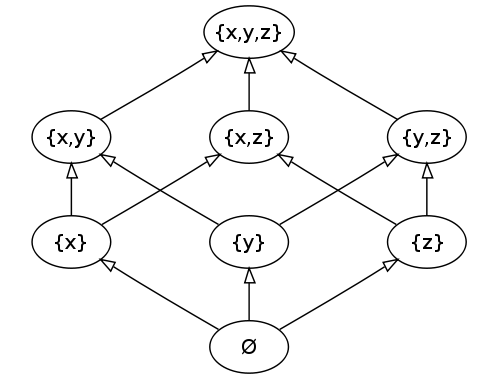
\includegraphics[scale=0.3]{img/Hasse_diagram_of_powerset_of_3.png}\end{center}
\end{document}